\chapter{Theoretical explanation}

\section{User experience (design)}
The official definition of user experience is: 
\begin{displayquote}
    A person's perception and responses resulting from the use and/or anticipated use of a product, system or service. (ISO 9241-11:2018, subsection 3.15).
\end{displayquote}

User experience \underline{design} is about making the user's experience with the product the best it can be. People who are interested should be attracted, once they are using the product, their journey should be as easy and pleasant as possible. To expose the needs of the user we should discover the behaviours, motivations and needs of the customer through observation, task analysis and other types of user feedback.

\subsection{UX Process}
    \subsubsection{User Personas}
    User personas are fictional characters, which are created based upon research in order to represent the different user types that might use your service, product, site or brand. As of today four different perspectives regarding personas exist. Only \underline{three} are related to this research.
    
    \paragraph{The goal-directed perspective}
        This perspective focuses on what the typical user wants to do with the product. As a \autoref{ux} researcher you want to examine the process a user would prefer to utilise in order to achieve their objectives. The goal-directed perspective is beautifully displayed in \autoref{fig:goal-directed-persona-perspective}. Author/Copyright holder: Smashing Magazine.
        \begin{figure}
            \centering
            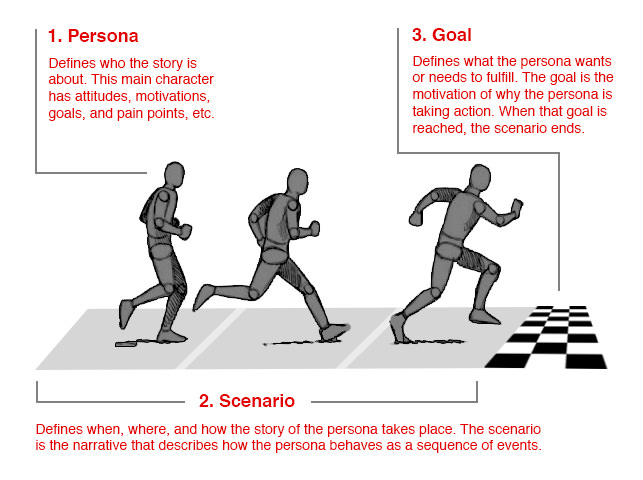
\includegraphics[scale=0.5]{goal-directed-perspective.jpg}
            \caption{Goal-directed persona perspective}
            \label{fig:goal-directed-persona-perspective}
        \end{figure}
    \paragraph{The role-based perspective}
    The role-based perspective is also a goal-directed perspective, but mainly focused on behavior. They are mainly focused on the role of the user inside the organization. A role-based persona should give an answer to the questions below.
    \begin{itemize}
        \item{Where will users use our product?}
        \item{What is the purpose of the product?}
        \item{What business objectives are required and what can be achieved with them?}
        \item{Which people will be impacted by its role?}
        \item{What kind of functions are being served..?}
    \end{itemize}
    
    \paragraph{The engaging perspective}
    Through an understanding of characters and stories, it is possible to create a realistic description of fictitious people. The engaging personas are designed so that the designers who use them can become more engaged with them. The more people engage with the persona and see them as 'real', the more likely they will be to consider them during the process design.
    
    \subsubsection{User Stories}
    Stories capture the characteristics of the design space and audience that designers and engineers need to understand to build a complete and useful software experience. A story is a design communication tool that transcends the cultural divides of multidisciplinary teams and intertwines a technology with its user's goals. This article describes how stories are powerful tools in software design, defines the elements that make a compelling story, and presents the use of stories at IBM from the authors' experience. It also explores the benefits at each phase of the design process and how stories evolve throughout the design process.
    \paragraph{User Flows}
    explanation about what user flows are
    
    \subsubsection{Research}
    \paragraph{mockups / wireframes}
    
    \subsubsection{Design}
    just some basic information about design
    
    \subsubsection{Implementation}
    information about the implementation
    
    \subsubsection{Evaluation}
    \paragraph{User feedback}
    \paragraph{UI audit reports}
    
\section{Data Analysis}
    \subsection{What is data analysis?}
    \subsection{What types of data analysis exists?}

\section{Generic interface}
    A major part of software engineering is building components that not only have a well-defined and consistent APIs, but are also very  \underline{reusable}. 
    \subsection{What is a generic interface}
    